\section{Metode}
\subsection{Utstyr}
\begin{itemize}
    \item Telefoner med Phyphox
    \item Telefonholder
    \item Trefot
    \item Vater
\end{itemize}
Det ble foretatt målinger med Djupviks iPhone SE, Jakobsens Samsung Galaxy A40 og Aakres iPhone 13. 

\subsection{Referansepunkter og målelokasjon}
Det ble gjort målinger med 2 ulike referansepunkt for å bedre datagrunnlag. De valgte referansepunktene var Nidarosdomen og Tyholttårnet, se figur 2\ref{fig:angle_north}. Koordinatene til referansepunktene ble bestemt via Google Maps. Koordinatene til målelokasjonen ble målt ved hjelp av Phyphox \cite{phyphox}. Telefonene ble kalibrert ved at de ble beveget noen meter i hver retning. Deretter ble de plassert i ro ved målelokasjon til målingen stabiliserte seg. Målingene ble utført på vestre siden av broen som krysser Eidsvolls gate langs Øvre alle. 


\subsection{Måling av magnetfelt og oppsett}
En trefot med en plattform for telefonene ble brukt, hvor telefonene ble plassert i en telefonholder. For å gi riktig retning på telefonene, ble det plassert ett vater langsmed telefonholderen \ref{fig:med_vater}. Vateret ble så brukt som siktemiddel slik at telefonholderen, og dermed telefonen lå i retning av referansepunktet. Deretter ble plattformen justert slik at den var horisontal ved hjelp av et vater.

Før hver måling ble telefonene kalibrert ved å spinne de rundt. Deretter ble telefonene plassert i telefonholderen og ble liggende der en tid til målingene var stabile. Dataene ble så eksportert. 

Måling med Nidarosdomen som referansepunkt ble gjennomført først. Detble kun gjennomført en måleserie. Deretter ble plattformen stilt inn på nytt, med Tyholttårnet som referansepunkt. Det ble gjort måling om flymodus og restarting av telefonene ville ha effekt. Målingene med flymodus ble gjennomført ved at telefonene ble satt i flymodus, kalibrert og dermed satt i telefonholderen. Målingene med restarting ble gjennomført ved at telefonene ble restartet, kalibrert og så plassert i telefonholderen.

For å finne posisjonen til målepunktet ble Phyphox benyttet. Da med «Location» som måling for GPS-koordinater. Telefonene ble kalibrert ved at de ble beveget noen meter i ulike retninger før selve målingen ble utført i telefonholderen. 
Dataene ble så analysert i Python ved hjelp av teorien beskrevet ovenfor, for å finne gjennomsnittsverdi, median og standardavvik for deklinasjonen og inklinasjonen for hver måleserie.     

 
\begin{figure}
    \centering
    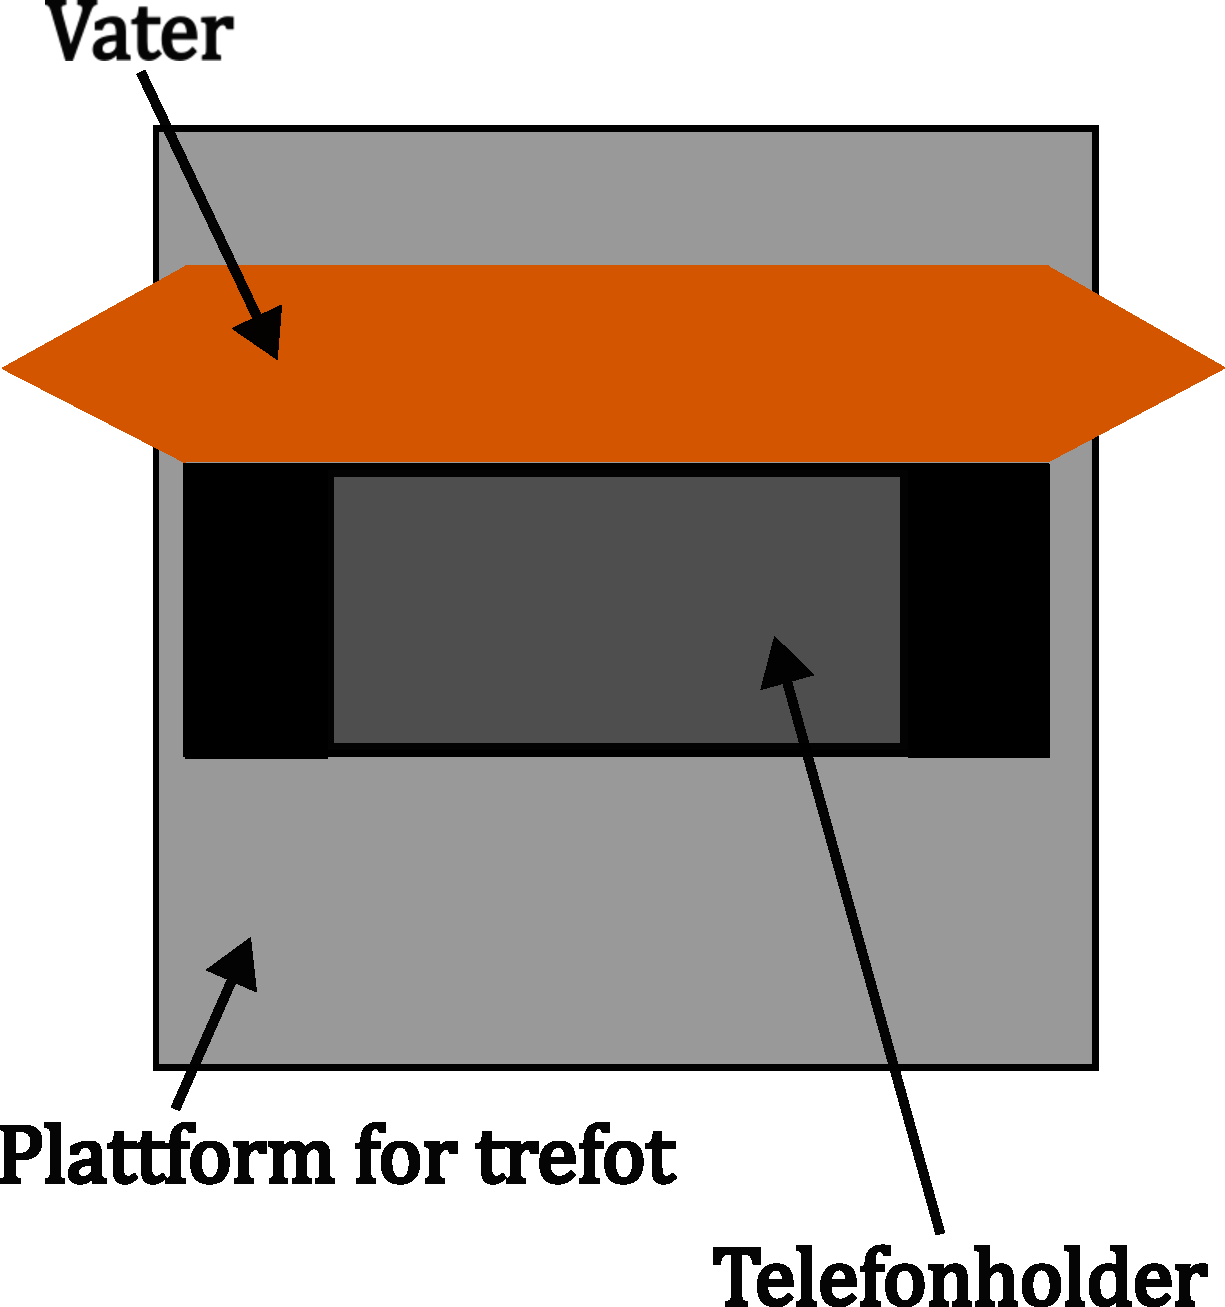
\includegraphics[width=0.45\textwidth]{img/Plattform med vater.pdf}                 
    \caption{Figuren viser oppsettet for måling før telefonen ble plassert i telefonholderen. Vateret er siktemiddel for referansepunktet.}
    \label{fig:med_vater}
\end{figure}

\begin{figure}
    \centering
    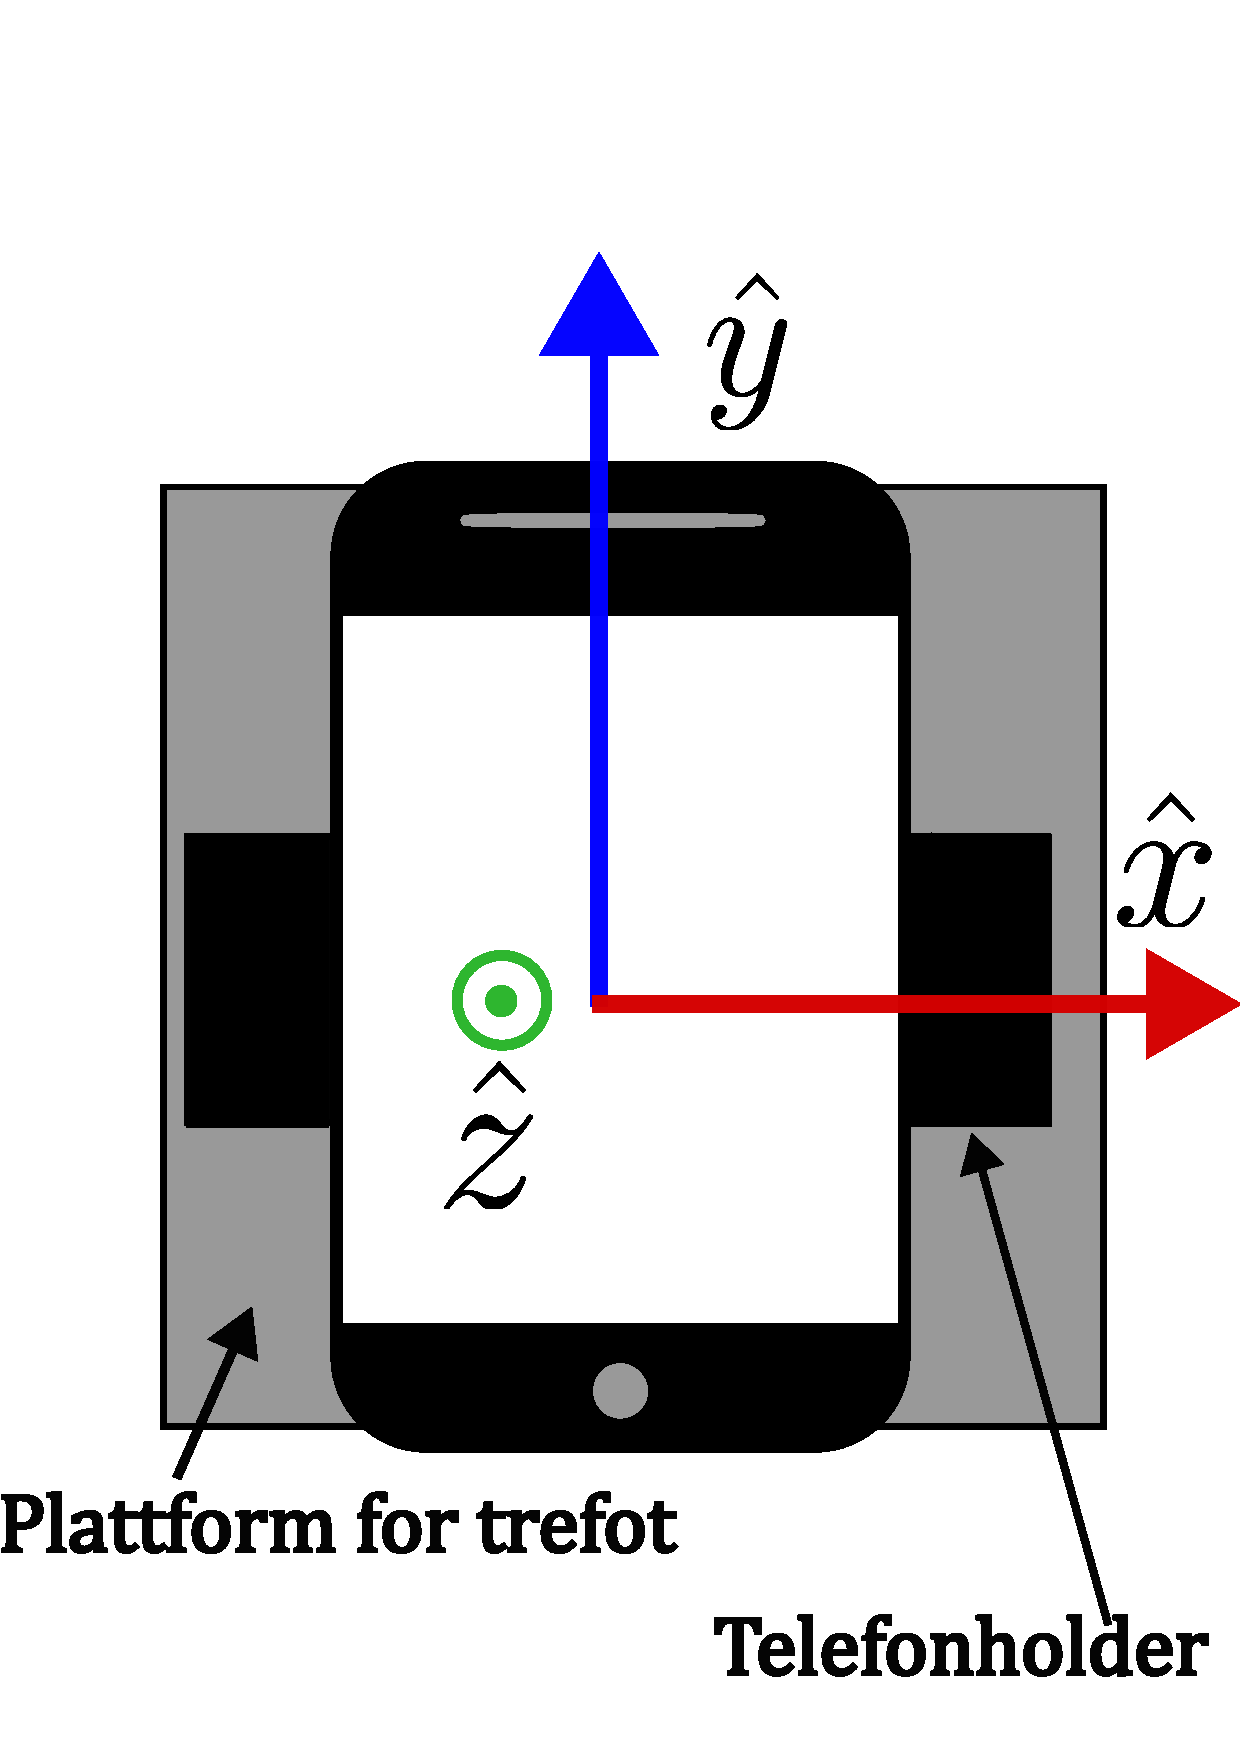
\includegraphics[width=0.65\textwidth]{img/Plattform med telefoni.pdf}
    \caption{Referansesystem for målinger foretatt med telefon satt i telefonholder.}
    \label{fig:telf_akser}
\end{figure}